% Options for packages loaded elsewhere
\PassOptionsToPackage{unicode}{hyperref}
\PassOptionsToPackage{hyphens}{url}
%
\documentclass[
]{book}
\usepackage{amsmath,amssymb}
\usepackage{lmodern}
\usepackage{iftex}
\ifPDFTeX
  \usepackage[T1]{fontenc}
  \usepackage[utf8]{inputenc}
  \usepackage{textcomp} % provide euro and other symbols
\else % if luatex or xetex
  \usepackage{unicode-math}
  \defaultfontfeatures{Scale=MatchLowercase}
  \defaultfontfeatures[\rmfamily]{Ligatures=TeX,Scale=1}
\fi
% Use upquote if available, for straight quotes in verbatim environments
\IfFileExists{upquote.sty}{\usepackage{upquote}}{}
\IfFileExists{microtype.sty}{% use microtype if available
  \usepackage[]{microtype}
  \UseMicrotypeSet[protrusion]{basicmath} % disable protrusion for tt fonts
}{}
\makeatletter
\@ifundefined{KOMAClassName}{% if non-KOMA class
  \IfFileExists{parskip.sty}{%
    \usepackage{parskip}
  }{% else
    \setlength{\parindent}{0pt}
    \setlength{\parskip}{6pt plus 2pt minus 1pt}}
}{% if KOMA class
  \KOMAoptions{parskip=half}}
\makeatother
\usepackage{xcolor}
\usepackage{color}
\usepackage{fancyvrb}
\newcommand{\VerbBar}{|}
\newcommand{\VERB}{\Verb[commandchars=\\\{\}]}
\DefineVerbatimEnvironment{Highlighting}{Verbatim}{commandchars=\\\{\}}
% Add ',fontsize=\small' for more characters per line
\usepackage{framed}
\definecolor{shadecolor}{RGB}{248,248,248}
\newenvironment{Shaded}{\begin{snugshade}}{\end{snugshade}}
\newcommand{\AlertTok}[1]{\textcolor[rgb]{0.94,0.16,0.16}{#1}}
\newcommand{\AnnotationTok}[1]{\textcolor[rgb]{0.56,0.35,0.01}{\textbf{\textit{#1}}}}
\newcommand{\AttributeTok}[1]{\textcolor[rgb]{0.77,0.63,0.00}{#1}}
\newcommand{\BaseNTok}[1]{\textcolor[rgb]{0.00,0.00,0.81}{#1}}
\newcommand{\BuiltInTok}[1]{#1}
\newcommand{\CharTok}[1]{\textcolor[rgb]{0.31,0.60,0.02}{#1}}
\newcommand{\CommentTok}[1]{\textcolor[rgb]{0.56,0.35,0.01}{\textit{#1}}}
\newcommand{\CommentVarTok}[1]{\textcolor[rgb]{0.56,0.35,0.01}{\textbf{\textit{#1}}}}
\newcommand{\ConstantTok}[1]{\textcolor[rgb]{0.00,0.00,0.00}{#1}}
\newcommand{\ControlFlowTok}[1]{\textcolor[rgb]{0.13,0.29,0.53}{\textbf{#1}}}
\newcommand{\DataTypeTok}[1]{\textcolor[rgb]{0.13,0.29,0.53}{#1}}
\newcommand{\DecValTok}[1]{\textcolor[rgb]{0.00,0.00,0.81}{#1}}
\newcommand{\DocumentationTok}[1]{\textcolor[rgb]{0.56,0.35,0.01}{\textbf{\textit{#1}}}}
\newcommand{\ErrorTok}[1]{\textcolor[rgb]{0.64,0.00,0.00}{\textbf{#1}}}
\newcommand{\ExtensionTok}[1]{#1}
\newcommand{\FloatTok}[1]{\textcolor[rgb]{0.00,0.00,0.81}{#1}}
\newcommand{\FunctionTok}[1]{\textcolor[rgb]{0.00,0.00,0.00}{#1}}
\newcommand{\ImportTok}[1]{#1}
\newcommand{\InformationTok}[1]{\textcolor[rgb]{0.56,0.35,0.01}{\textbf{\textit{#1}}}}
\newcommand{\KeywordTok}[1]{\textcolor[rgb]{0.13,0.29,0.53}{\textbf{#1}}}
\newcommand{\NormalTok}[1]{#1}
\newcommand{\OperatorTok}[1]{\textcolor[rgb]{0.81,0.36,0.00}{\textbf{#1}}}
\newcommand{\OtherTok}[1]{\textcolor[rgb]{0.56,0.35,0.01}{#1}}
\newcommand{\PreprocessorTok}[1]{\textcolor[rgb]{0.56,0.35,0.01}{\textit{#1}}}
\newcommand{\RegionMarkerTok}[1]{#1}
\newcommand{\SpecialCharTok}[1]{\textcolor[rgb]{0.00,0.00,0.00}{#1}}
\newcommand{\SpecialStringTok}[1]{\textcolor[rgb]{0.31,0.60,0.02}{#1}}
\newcommand{\StringTok}[1]{\textcolor[rgb]{0.31,0.60,0.02}{#1}}
\newcommand{\VariableTok}[1]{\textcolor[rgb]{0.00,0.00,0.00}{#1}}
\newcommand{\VerbatimStringTok}[1]{\textcolor[rgb]{0.31,0.60,0.02}{#1}}
\newcommand{\WarningTok}[1]{\textcolor[rgb]{0.56,0.35,0.01}{\textbf{\textit{#1}}}}
\usepackage{longtable,booktabs,array}
\usepackage{calc} % for calculating minipage widths
% Correct order of tables after \paragraph or \subparagraph
\usepackage{etoolbox}
\makeatletter
\patchcmd\longtable{\par}{\if@noskipsec\mbox{}\fi\par}{}{}
\makeatother
% Allow footnotes in longtable head/foot
\IfFileExists{footnotehyper.sty}{\usepackage{footnotehyper}}{\usepackage{footnote}}
\makesavenoteenv{longtable}
\usepackage{graphicx}
\makeatletter
\def\maxwidth{\ifdim\Gin@nat@width>\linewidth\linewidth\else\Gin@nat@width\fi}
\def\maxheight{\ifdim\Gin@nat@height>\textheight\textheight\else\Gin@nat@height\fi}
\makeatother
% Scale images if necessary, so that they will not overflow the page
% margins by default, and it is still possible to overwrite the defaults
% using explicit options in \includegraphics[width, height, ...]{}
\setkeys{Gin}{width=\maxwidth,height=\maxheight,keepaspectratio}
% Set default figure placement to htbp
\makeatletter
\def\fps@figure{htbp}
\makeatother
\setlength{\emergencystretch}{3em} % prevent overfull lines
\providecommand{\tightlist}{%
  \setlength{\itemsep}{0pt}\setlength{\parskip}{0pt}}
\setcounter{secnumdepth}{5}
\usepackage{booktabs}
\ifLuaTeX
  \usepackage{selnolig}  % disable illegal ligatures
\fi
\usepackage[]{natbib}
\bibliographystyle{apalike}
\IfFileExists{bookmark.sty}{\usepackage{bookmark}}{\usepackage{hyperref}}
\IfFileExists{xurl.sty}{\usepackage{xurl}}{} % add URL line breaks if available
\urlstyle{same} % disable monospaced font for URLs
\hypersetup{
  pdftitle={NIvis},
  hidelinks,
  pdfcreator={LaTeX via pandoc}}

\title{NIvis}
\author{}
\date{\vspace{-2.5em}2022-10-14}

\begin{document}
\maketitle

{
\setcounter{tocdepth}{1}
\tableofcontents
}
\hypertarget{introduction}{%
\chapter{Introduction}\label{introduction}}

\hypertarget{downloading-and-prepaering-example-data}{%
\chapter{Downloading and prepaering example data}\label{downloading-and-prepaering-example-data}}

\hypertarget{cross}{%
\chapter{Time series}\label{cross}}

\hypertarget{raw-data}{%
\section{Raw data}\label{raw-data}}

\hypertarget{scaled-data}{%
\section{Scaled data}\label{scaled-data}}

\hypertarget{maps}{%
\chapter{Maps}\label{maps}}

\hypertarget{raw-data-1}{%
\section{Raw data}\label{raw-data-1}}

\hypertarget{scaled-data-1}{%
\section{Scaled data}\label{scaled-data-1}}

\hypertarget{jerv}{%
\subsection{Jerv}\label{jerv}}

\hypertarget{prepare-ni-data}{%
\subsubsection{Prepare NI data}\label{prepare-ni-data}}

The jerv (wolverine) data was downloaded using the \texttt{R/singleIndicator.R} script and the importDatasetApi() function,, and subsequently the assembleNiObject() function, so now I can simply import it.

\begin{Shaded}
\begin{Highlighting}[]
\NormalTok{jerv }\OtherTok{\textless{}{-}} \FunctionTok{readRDS}\NormalTok{(}\StringTok{"data/jerv\_assemble.rds"}\NormalTok{)}
\end{Highlighting}
\end{Shaded}

This data file contains the raw data in the form of expected values for each BSunits (municipalities). But we actually want to keep the original geometeris of the eight rovviltregioner, and so we need to focus in the ICunits instead.

\begin{Shaded}
\begin{Highlighting}[]
\FunctionTok{par}\NormalTok{(}\AttributeTok{mar=}\FunctionTok{c}\NormalTok{(}\DecValTok{9}\NormalTok{,}\DecValTok{5}\NormalTok{,}\DecValTok{1}\NormalTok{,}\DecValTok{1}\NormalTok{))}
\FunctionTok{barplot}\NormalTok{(jerv}\SpecialCharTok{$}\NormalTok{indicatorValues}\SpecialCharTok{$}\StringTok{\textasciigrave{}}\AttributeTok{2019}\StringTok{\textasciigrave{}}\SpecialCharTok{$}\NormalTok{expectedValue,}
        \AttributeTok{names.arg =}\NormalTok{ jerv}\SpecialCharTok{$}\NormalTok{indicatorValues}\SpecialCharTok{$}\StringTok{\textasciigrave{}}\AttributeTok{2019}\StringTok{\textasciigrave{}}\SpecialCharTok{$}\NormalTok{ICunitName, }
        \AttributeTok{las=}\DecValTok{2}\NormalTok{,}
        \AttributeTok{ylab =} \StringTok{"Estimated number of}\SpecialCharTok{\textbackslash{}n}\StringTok{wolverine in 2019"}\NormalTok{)}
\end{Highlighting}
\end{Shaded}

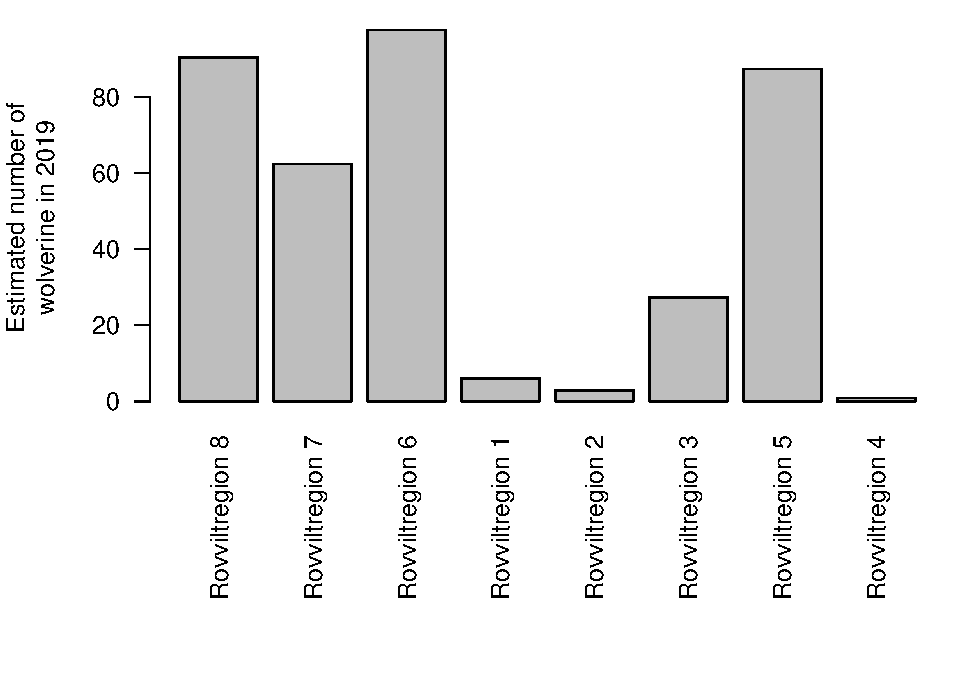
\includegraphics{03-maps_files/figure-latex/unnamed-chunk-3-1.pdf}

The data also contains upper and lower quantiles, but we can also get the full probability distribution and sample from it to get standard deviations.
but also as probability functions that we can sample from:

\begin{Shaded}
\begin{Highlighting}[]
\CommentTok{\# bruker tradOb siden custumDist er NA. Dette er ikke en generisk løsning. }
\NormalTok{obstype }\OtherTok{\textless{}{-}} \FunctionTok{rep}\NormalTok{(}\StringTok{"tradObs"}\NormalTok{, }\FunctionTok{nrow}\NormalTok{(jerv}\SpecialCharTok{$}\NormalTok{indicatorValues}\SpecialCharTok{$}\StringTok{\textquotesingle{}2019\textquotesingle{}}\NormalTok{))}

\CommentTok{\#myYears \textless{}{-} as.character(c(1990,2000,2010,2014,2019))}
\NormalTok{myYears }\OtherTok{\textless{}{-}} \FunctionTok{as.character}\NormalTok{(}\FunctionTok{c}\NormalTok{(}\DecValTok{2019}\NormalTok{))}

\ControlFlowTok{for}\NormalTok{(i }\ControlFlowTok{in} \DecValTok{1}\SpecialCharTok{:}\FunctionTok{length}\NormalTok{(myYears))\{}
\CommentTok{\# print(i)}

\NormalTok{myMat }\OtherTok{\textless{}{-}}\NormalTok{ NIcalc}\SpecialCharTok{::}\FunctionTok{sampleObsMat}\NormalTok{(}
  \AttributeTok{ICunitId           =}\NormalTok{ jerv}\SpecialCharTok{$}\NormalTok{indicatorValues[[i]]}\SpecialCharTok{$}\NormalTok{ICunitId, }
  \AttributeTok{value              =}\NormalTok{ jerv}\SpecialCharTok{$}\NormalTok{indicatorValues[[i]]}\SpecialCharTok{$}\NormalTok{expectedValue,}
  \AttributeTok{distrib            =}\NormalTok{ jerv}\SpecialCharTok{$}\NormalTok{indicatorValues[[i]]}\SpecialCharTok{$}\NormalTok{distributionFamilyName,}
  \AttributeTok{mu                 =}\NormalTok{ jerv}\SpecialCharTok{$}\NormalTok{indicatorValues[[i]]}\SpecialCharTok{$}\NormalTok{distParameter1,}
  \AttributeTok{sig                =}\NormalTok{ jerv}\SpecialCharTok{$}\NormalTok{indicatorValues[[i]]}\SpecialCharTok{$}\NormalTok{distParameter2,}
  \AttributeTok{customDistribution =}\NormalTok{ jerv}\SpecialCharTok{$}\NormalTok{indicatorValues[[i]]}\SpecialCharTok{$}\NormalTok{customDistribution,}
          \AttributeTok{obsType =}\NormalTok{ obstype,}
          \AttributeTok{nsim =} \DecValTok{1000}
          
\NormalTok{)}
\FunctionTok{assign}\NormalTok{(}\FunctionTok{paste0}\NormalTok{(}\StringTok{"myMat"}\NormalTok{, myYears[i]), myMat)}
\NormalTok{\}}
\CommentTok{\#\textgreater{} Warning: replacing previous import \textquotesingle{}distr::plot\textquotesingle{} by}
\CommentTok{\#\textgreater{} \textquotesingle{}graphics::plot\textquotesingle{} when loading \textquotesingle{}NIcalc\textquotesingle{}}

\FunctionTok{par}\NormalTok{(}\AttributeTok{mfrow =} \FunctionTok{c}\NormalTok{(}\DecValTok{1}\NormalTok{,}\DecValTok{2}\NormalTok{))}
\FunctionTok{hist}\NormalTok{(myMat2019[}\DecValTok{1}\NormalTok{,], }\AttributeTok{main =} \StringTok{"Rovviltregion 1"}\NormalTok{, }\AttributeTok{xlab =} \StringTok{""}\NormalTok{)}
\FunctionTok{hist}\NormalTok{(myMat2019[}\DecValTok{8}\NormalTok{,], }\AttributeTok{main =} \StringTok{"Rovviltregion 8"}\NormalTok{, }\AttributeTok{xlab =} \StringTok{""}\NormalTok{)}
\end{Highlighting}
\end{Shaded}

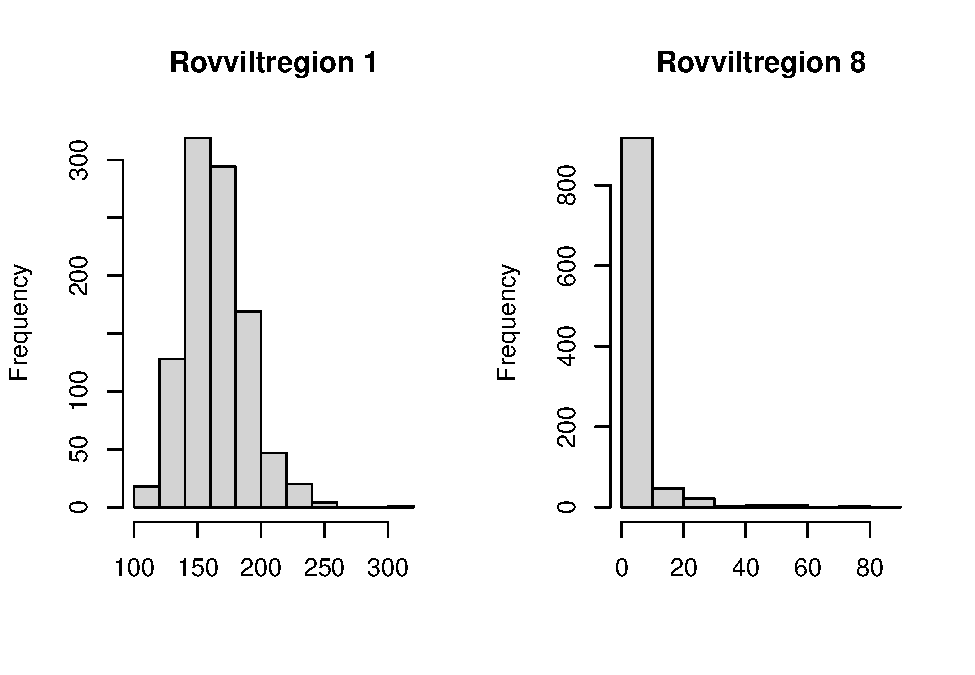
\includegraphics{03-maps_files/figure-latex/unnamed-chunk-4-1.pdf}

For some reason the extected values are far from the mean of these distributions. I did this exercise \href{https://ninanor.github.io/IBECA/jerv.html}{once before}, and did not get this problem then. I think the difference is that I use eco = NULL this time, in the \texttt{importDatasetApi()}, and this cause the output to somehow split into forest and alpine ecosystems. I will ignore this here for this example.

I can also get the reference values in the same way, and then divide one by the other to get scaled values

\begin{Shaded}
\begin{Highlighting}[]
\NormalTok{myMatr }\OtherTok{\textless{}{-}}\NormalTok{ NIcalc}\SpecialCharTok{::}\FunctionTok{sampleObsMat}\NormalTok{(}
\NormalTok{            jerv}\SpecialCharTok{$}\NormalTok{referenceValues}\SpecialCharTok{$}\NormalTok{ICunitId, }
\NormalTok{            jerv}\SpecialCharTok{$}\NormalTok{referenceValues}\SpecialCharTok{$}\NormalTok{expectedValue,}
\NormalTok{            jerv}\SpecialCharTok{$}\NormalTok{referenceValues}\SpecialCharTok{$}\NormalTok{distributionFamilyName,}
            \AttributeTok{mu =}\NormalTok{ jerv}\SpecialCharTok{$}\NormalTok{referenceValues}\SpecialCharTok{$}\NormalTok{distParameter1,}
            \AttributeTok{sig =}\NormalTok{ jerv}\SpecialCharTok{$}\NormalTok{referenceValues}\SpecialCharTok{$}\NormalTok{distParameter2,}
            \AttributeTok{customDistribution =}\NormalTok{ jerv}\SpecialCharTok{$}\NormalTok{referenceValues}\SpecialCharTok{$}\NormalTok{customDistribution,}
            \AttributeTok{obsType =}\NormalTok{ obstype,}
            \AttributeTok{nsim =}\DecValTok{1000}
\NormalTok{        )}

\NormalTok{temp }\OtherTok{\textless{}{-}} \FunctionTok{colSums}\NormalTok{(myMat2019)}\SpecialCharTok{/}\FunctionTok{colSums}\NormalTok{(myMatr)}
\FunctionTok{hist}\NormalTok{(temp)}
\end{Highlighting}
\end{Shaded}

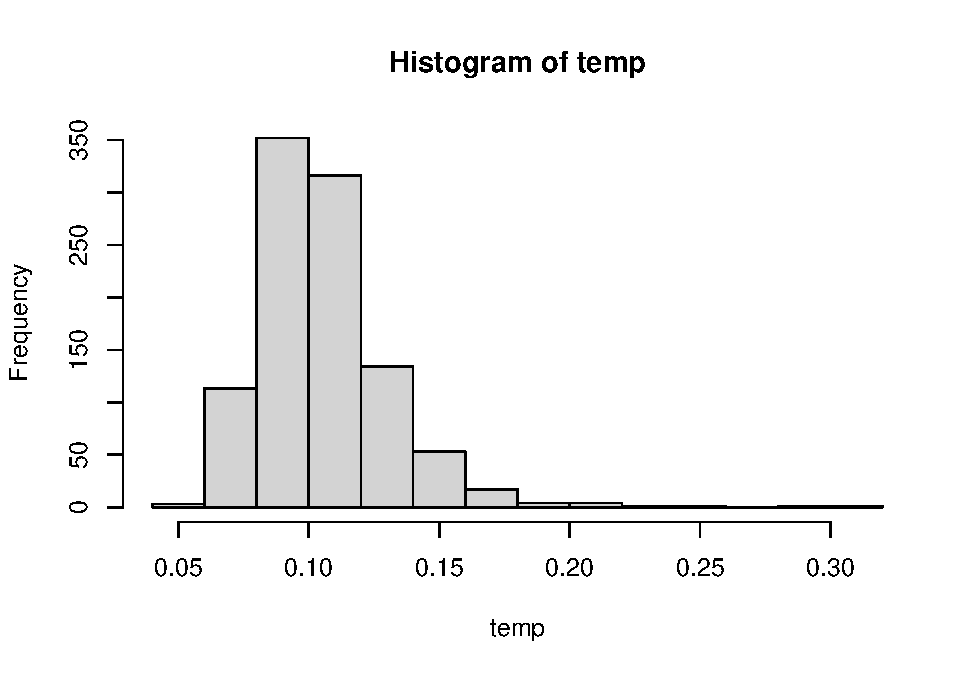
\includegraphics{03-maps_files/figure-latex/unnamed-chunk-5-1.pdf}

Then I will create a data frame with the mean indicator values and the SD.

\begin{Shaded}
\begin{Highlighting}[]
\FunctionTok{library}\NormalTok{(matrixStats)}
\CommentTok{\#\textgreater{} Warning: package \textquotesingle{}matrixStats\textquotesingle{} was built under R version}
\CommentTok{\#\textgreater{} 4.1.3}
\NormalTok{jerv\_tbl }\OtherTok{\textless{}{-}} \FunctionTok{data.frame}\NormalTok{(}\StringTok{"raw2019"} \OtherTok{=} \FunctionTok{round}\NormalTok{(}\FunctionTok{rowMeans}\NormalTok{(myMat2019), }\DecValTok{2}\NormalTok{),}
                       \StringTok{"sd2019"}  \OtherTok{=} \FunctionTok{round}\NormalTok{(matrixStats}\SpecialCharTok{::}\FunctionTok{rowSds}\NormalTok{(myMat2019), }\DecValTok{2}\NormalTok{),}
                       \StringTok{"ref"}     \OtherTok{=} \FunctionTok{round}\NormalTok{(}\FunctionTok{rowMeans}\NormalTok{(myMatr), }\DecValTok{2}\NormalTok{))}
\NormalTok{jerv\_tbl}\SpecialCharTok{$}\NormalTok{scaled }\OtherTok{\textless{}{-}} \FunctionTok{round}\NormalTok{(jerv\_tbl}\SpecialCharTok{$}\NormalTok{raw2019}\SpecialCharTok{/}\NormalTok{jerv\_tbl}\SpecialCharTok{$}\NormalTok{ref, }\DecValTok{2}\NormalTok{)}
\NormalTok{jerv\_tbl}\SpecialCharTok{$}\NormalTok{cv }\OtherTok{\textless{}{-}} \FunctionTok{round}\NormalTok{(jerv\_tbl}\SpecialCharTok{$}\NormalTok{sd2019}\SpecialCharTok{/}\NormalTok{jerv\_tbl}\SpecialCharTok{$}\NormalTok{raw2019, }\DecValTok{2}\NormalTok{)}
\NormalTok{jerv\_tbl}\SpecialCharTok{$}\NormalTok{region }\OtherTok{\textless{}{-}}\NormalTok{ jerv}\SpecialCharTok{$}\NormalTok{indicatorValues}\SpecialCharTok{$}\StringTok{\textasciigrave{}}\AttributeTok{2019}\StringTok{\textasciigrave{}}\SpecialCharTok{$}\NormalTok{ICunitName}
\NormalTok{DT}\SpecialCharTok{::}\FunctionTok{datatable}\NormalTok{(jerv\_tbl)}
\end{Highlighting}
\end{Shaded}

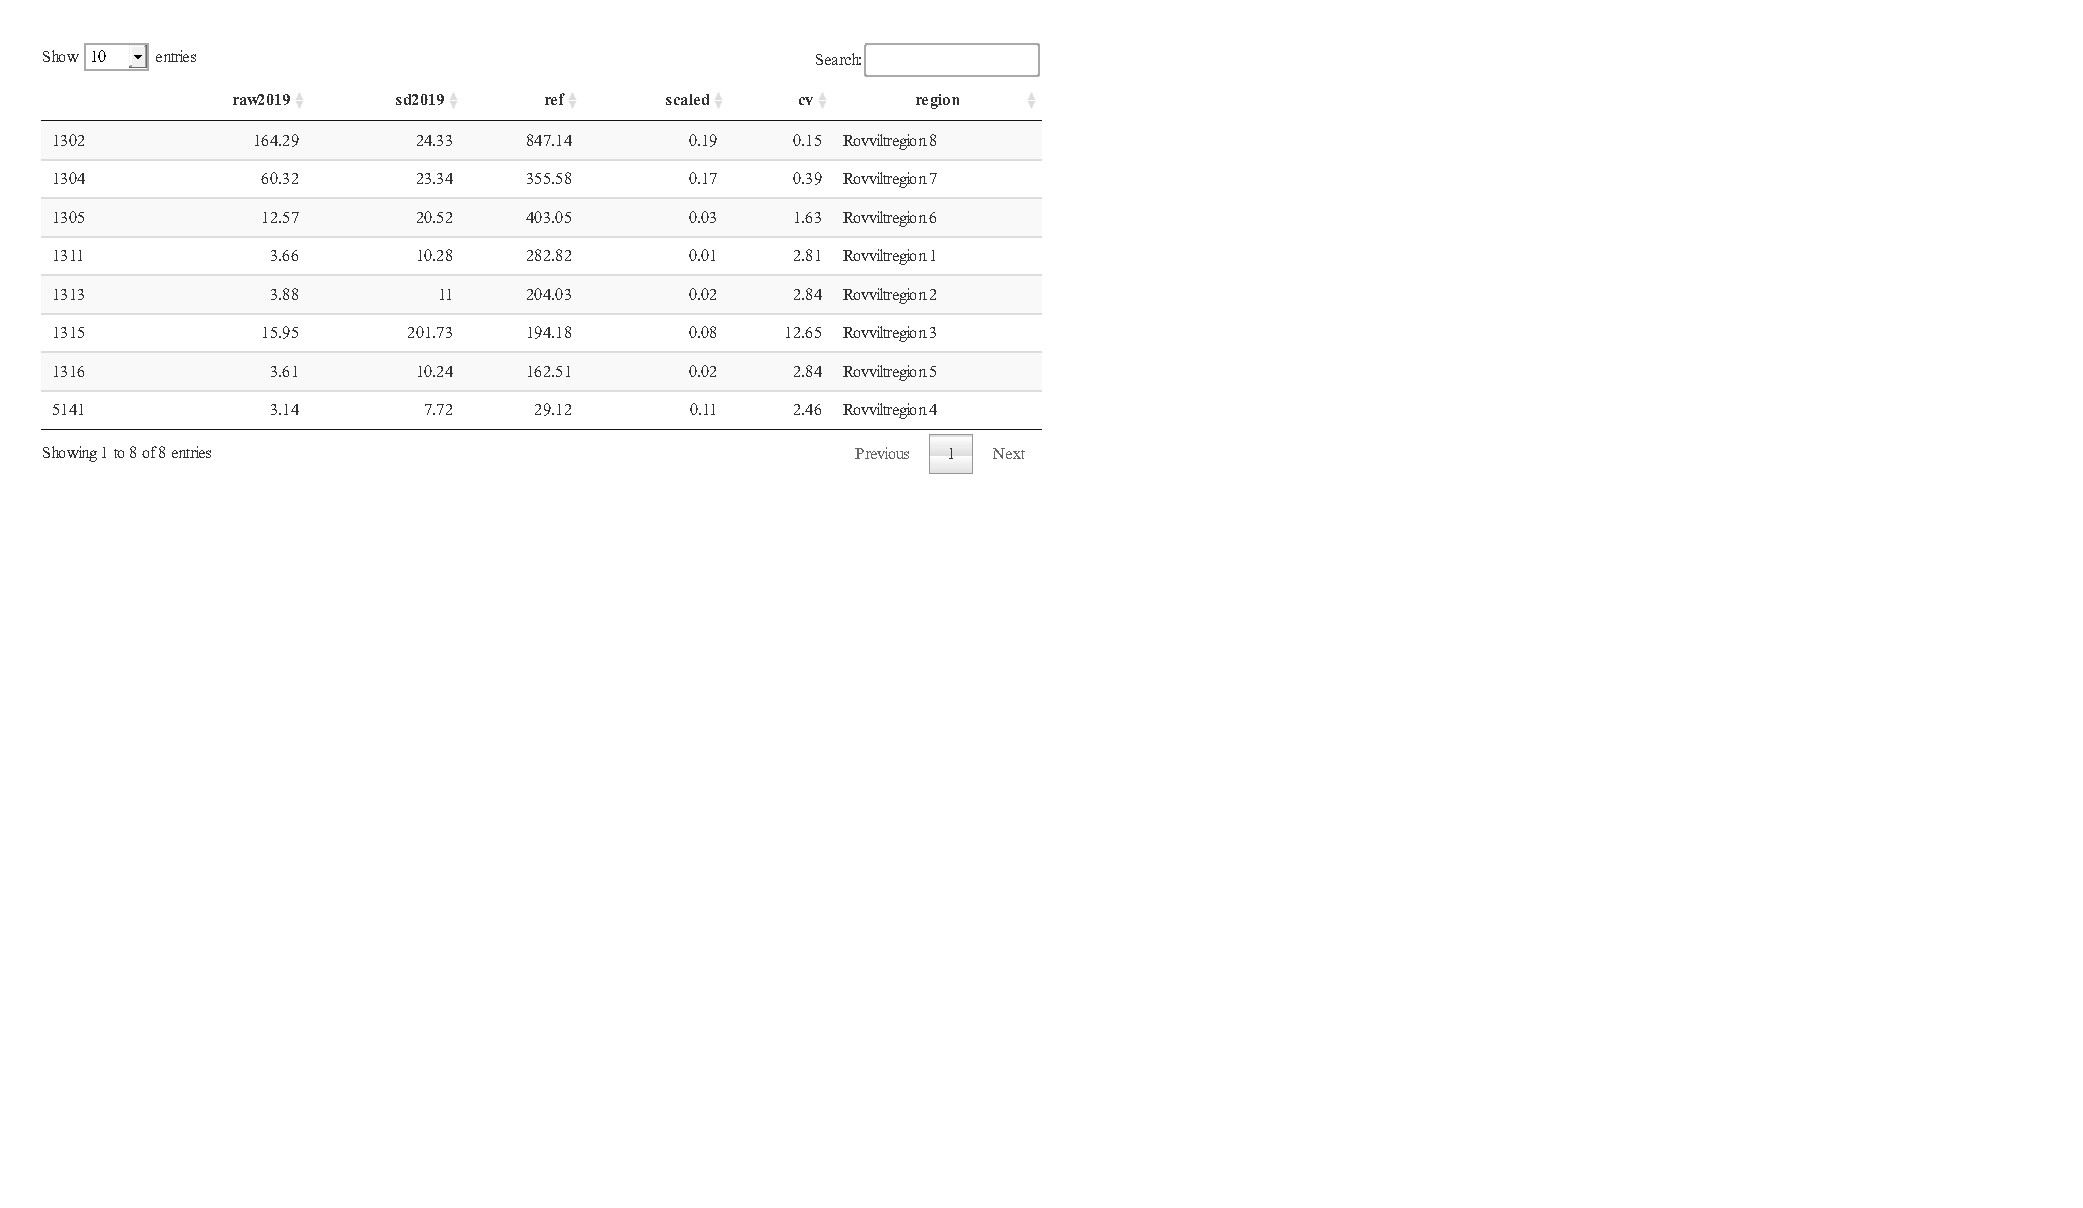
\includegraphics{03-maps_files/figure-latex/unnamed-chunk-6-1.pdf}
This is a special case maybe, because the sd is often larger than the mean.

Btw, we could use inbuilt NIcalc functions to get the indicator value, like I do below, but that will aggregate to regions, and we want to keep the original geometry.

\begin{Shaded}
\begin{Highlighting}[]
\NormalTok{jervComp }\OtherTok{\textless{}{-}}\NormalTok{ NIcalc}\SpecialCharTok{::}\FunctionTok{calculateIndex}\NormalTok{(}
  \AttributeTok{x       =}\NormalTok{ jerv,}
  \AttributeTok{nsim     =} \DecValTok{1000}\NormalTok{,}
  \AttributeTok{awBSunit =} \StringTok{"terrestrialArea"}\NormalTok{,}
  \AttributeTok{fids     =}\NormalTok{ F,    }\CommentTok{\# should fidelities be ignored in }
                   \CommentTok{\# the calculation of Wi?}
  \AttributeTok{tgroups  =}\NormalTok{ F, }\CommentTok{\# should grouping of indicators }
                   \CommentTok{\# into trophic and key indicator }
                   \CommentTok{\# groups be ignored}
  \AttributeTok{keys     =} \StringTok{"specialWeight"}\NormalTok{, }\CommentTok{\#"ignore",}
\NormalTok{)}
\CommentTok{\#\textgreater{} Indices for NIunits \textquotesingle{}wholeArea\textquotesingle{}, \textquotesingle{}E\textquotesingle{}, \textquotesingle{}S\textquotesingle{}, \textquotesingle{}W\textquotesingle{}, \textquotesingle{}C\textquotesingle{}, \textquotesingle{}N\textquotesingle{}}
\CommentTok{\#\textgreater{} and years \textquotesingle{}1990\textquotesingle{}, \textquotesingle{}2000\textquotesingle{}, \textquotesingle{}2010\textquotesingle{}, \textquotesingle{}2014\textquotesingle{}, \textquotesingle{}2019\textquotesingle{} will be calculated.}
\CommentTok{\#\textgreater{} The 30 index distributions will each be based on  1000 simulations.}
\CommentTok{\#\textgreater{} There are 8 ICunits with observations in data set \textquotesingle{}jerv\textquotesingle{}.}
\CommentTok{\#\textgreater{} }
\CommentTok{\#\textgreater{} Calculating weights that are the same for all years .....}
\CommentTok{\#\textgreater{} }
\CommentTok{\#\textgreater{} Sampling reference values .....}
\CommentTok{\#\textgreater{} }
\CommentTok{\#\textgreater{} Sampling and scaling indicator observations from  1990 .....}
\CommentTok{\#\textgreater{} }
\CommentTok{\#\textgreater{} Sampling and scaling indicator observations from  2000 .....}
\CommentTok{\#\textgreater{} }
\CommentTok{\#\textgreater{} Sampling and scaling indicator observations from  2010 .....}
\CommentTok{\#\textgreater{} }
\CommentTok{\#\textgreater{} Sampling and scaling indicator observations from  2014 .....}
\CommentTok{\#\textgreater{} }
\CommentTok{\#\textgreater{} Sampling and scaling indicator observations from  2019 .....}
\FunctionTok{plot}\NormalTok{(jervComp}\SpecialCharTok{$}\NormalTok{wholeArea)}
\end{Highlighting}
\end{Shaded}

\begin{figure}
\centering
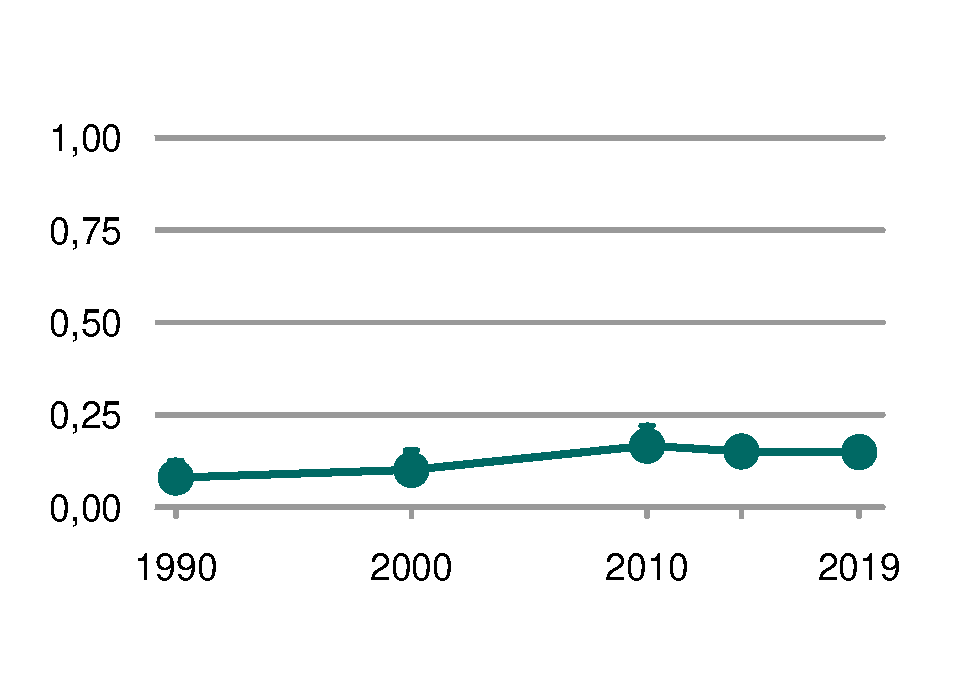
\includegraphics{03-maps_files/figure-latex/unnamed-chunk-7-1.pdf}
\caption{\label{fig:unnamed-chunk-7}The scaled indicator values for wolverine across Norway.}
\end{figure}

\hypertarget{get-geometries}{%
\subsubsection{Get geometries}\label{get-geometries}}

Then I can get the spatial geometries associated with the data. There are the so called rovviltregioner. There are eight of them. They are actually linked to the BS-units (municipalites), but we don't want to plot the outlines of the municipalities.

\emph{Add text about how we got the json file and converted it to a shape file}

\begin{Shaded}
\begin{Highlighting}[]
\NormalTok{path }\OtherTok{\textless{}{-}} \StringTok{"P:/41201612\_naturindeks\_2021\_2023\_database\_og\_innsynslosning/Pilot\_Forbedring\_Innsynsløsning/Shapefiles/Jerv"}
\end{Highlighting}
\end{Shaded}

\begin{Shaded}
\begin{Highlighting}[]
\FunctionTok{library}\NormalTok{(sf)}
\CommentTok{\#\textgreater{} Linking to GEOS 3.9.1, GDAL 3.2.1, PROJ 7.2.1; sf\_use\_s2() is TRUE}
\NormalTok{rov }\OtherTok{\textless{}{-}}\NormalTok{ sf}\SpecialCharTok{::}\FunctionTok{read\_sf}\NormalTok{(path)}
\NormalTok{rov }\OtherTok{\textless{}{-}}\NormalTok{ sf}\SpecialCharTok{::}\FunctionTok{st\_make\_valid}\NormalTok{(rov)}
\NormalTok{rov }\OtherTok{\textless{}{-}}\NormalTok{ rov[rov}\SpecialCharTok{$}\NormalTok{area}\SpecialCharTok{!=}\StringTok{"DEF jerv"}\NormalTok{,]}
\end{Highlighting}
\end{Shaded}

Clip it against the outline of Norway to make it look more pretty

\begin{Shaded}
\begin{Highlighting}[]
\NormalTok{path }\OtherTok{\textless{}{-}} \StringTok{"data/outlineOfNorway\_EPSG25833.shp"}
\NormalTok{nor }\OtherTok{\textless{}{-}}\NormalTok{ sf}\SpecialCharTok{::}\FunctionTok{read\_sf}\NormalTok{(path)}
\NormalTok{nor }\OtherTok{\textless{}{-}} \FunctionTok{st\_transform}\NormalTok{(nor, }\AttributeTok{crs=}\FunctionTok{st\_crs}\NormalTok{(rov))}
\end{Highlighting}
\end{Shaded}

\begin{Shaded}
\begin{Highlighting}[]
\NormalTok{rov }\OtherTok{\textless{}{-}} \FunctionTok{st\_intersection}\NormalTok{(rov, nor)}
\CommentTok{\#\textgreater{} Warning: attribute variables are assumed to be spatially}
\CommentTok{\#\textgreater{} constant throughout all geometries}
\end{Highlighting}
\end{Shaded}

\hypertarget{link-data-and-geometries}{%
\subsubsection{Link data and geometries}\label{link-data-and-geometries}}

\begin{Shaded}
\begin{Highlighting}[]
\NormalTok{rov}\SpecialCharTok{$}\NormalTok{scaledIndicator }\OtherTok{\textless{}{-}}\NormalTok{ jerv\_tbl}\SpecialCharTok{$}\NormalTok{scaled[}\FunctionTok{match}\NormalTok{(rov}\SpecialCharTok{$}\NormalTok{area, jerv\_tbl}\SpecialCharTok{$}\NormalTok{region)]}
\NormalTok{rov}\SpecialCharTok{$}\NormalTok{cv }\OtherTok{\textless{}{-}}\NormalTok{ jerv\_tbl}\SpecialCharTok{$}\NormalTok{cv[}\FunctionTok{match}\NormalTok{(rov}\SpecialCharTok{$}\NormalTok{area, jerv\_tbl}\SpecialCharTok{$}\NormalTok{region)]}
\NormalTok{rov}\SpecialCharTok{$}\NormalTok{raw }\OtherTok{\textless{}{-}}\NormalTok{ jerv\_tbl}\SpecialCharTok{$}\NormalTok{raw2019[}\FunctionTok{match}\NormalTok{(rov}\SpecialCharTok{$}\NormalTok{area, jerv\_tbl}\SpecialCharTok{$}\NormalTok{region)]}
\end{Highlighting}
\end{Shaded}

\begin{Shaded}
\begin{Highlighting}[]
\FunctionTok{library}\NormalTok{(tmap)}
\NormalTok{one }\OtherTok{\textless{}{-}} \FunctionTok{tm\_shape}\NormalTok{(rov)}\SpecialCharTok{+}
  \FunctionTok{tm\_polygons}\NormalTok{(}\AttributeTok{col=}\StringTok{"scaledIndicator"}\NormalTok{, }
              \AttributeTok{border.col =} \StringTok{"white"}\NormalTok{)}

\NormalTok{two }\OtherTok{\textless{}{-}} \FunctionTok{tm\_shape}\NormalTok{(rov)}\SpecialCharTok{+}
  \FunctionTok{tm\_polygons}\NormalTok{(}\AttributeTok{col=}\StringTok{"cv"}\NormalTok{, }
              \AttributeTok{border.col =} \StringTok{"white"}\NormalTok{)}

\NormalTok{three }\OtherTok{\textless{}{-}} \FunctionTok{tm\_shape}\NormalTok{(rov)}\SpecialCharTok{+}
  \FunctionTok{tm\_polygons}\NormalTok{(}\AttributeTok{col=}\StringTok{"raw"}\NormalTok{, }
              \AttributeTok{border.col =} \StringTok{"white"}\NormalTok{)}


\FunctionTok{tmap\_arrange}\NormalTok{(one, two, }
             \AttributeTok{widths =} \FunctionTok{c}\NormalTok{(.}\DecValTok{75}\NormalTok{, .}\DecValTok{25}\NormalTok{),}
             \AttributeTok{heights =} \FunctionTok{c}\NormalTok{(}\DecValTok{1}\NormalTok{, }\FloatTok{0.5}\NormalTok{))}
\CommentTok{\#\textgreater{} Some legend labels were too wide. These labels have been resized to 0.61, 0.53, 0.53. Increase legend.width (argument of tm\_layout) to make the legend wider and therefore the labels larger.}
\end{Highlighting}
\end{Shaded}

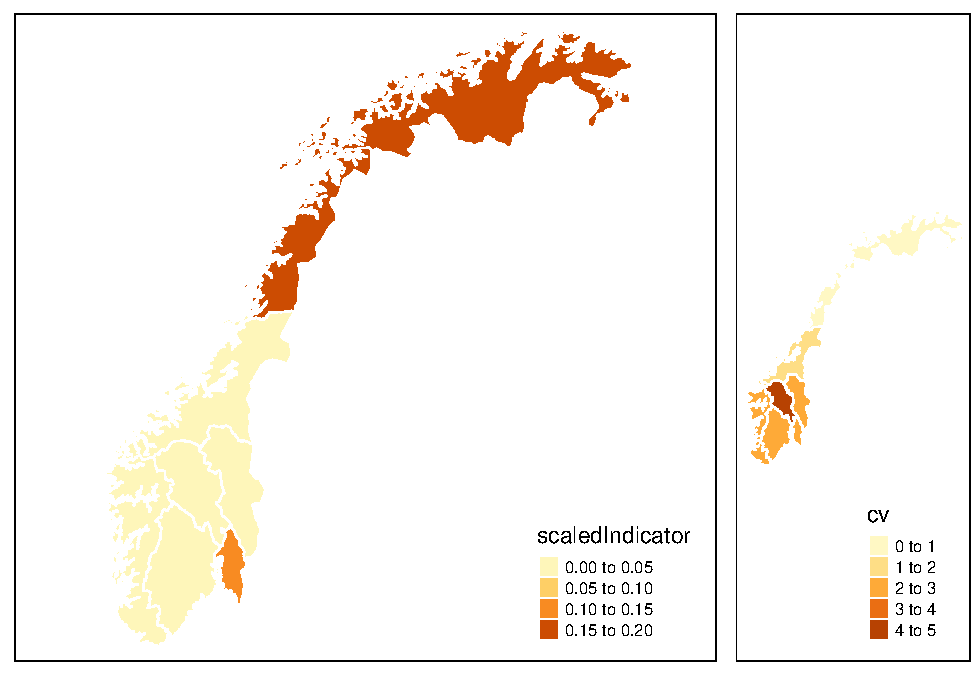
\includegraphics{03-maps_files/figure-latex/unnamed-chunk-13-1.pdf}

\hypertarget{other-figures}{%
\chapter{Other figures}\label{other-figures}}

  \bibliography{book.bib,packages.bib}

\end{document}
